%%%%%%%%%%%%%%%%%%%%%%%%%%%%%%%%%%%%%%%%%%%%%%%%%%%%%%%%
% LabOrTool - Laboratory Organization Tool
% Copyright (C) 2014-2015 Marco Giammarini
%
% Author(s):
%  Marco Giammarini <m.giammarini@warcomeb.it>
%
% This program is free software: you can redistribute it and/or modify
% it under the terms of the GNU General Public License as published by
% the Free Software Foundation, either version 3 of the License, or
% any later version.
%
% This program is distributed in the hope that it will be useful,
% but WITHOUT ANY WARRANTY; without even the implied warranty of
% MERCHANTABILITY or FITNESS FOR A PARTICULAR PURPOSE.  See the
% GNU General Public License for more details.
%
% You should have received a copy of the GNU General Public License
% along with this program. If not, see <http://www.gnu.org/licenses/>
%
% The compiled version of this file is licensed under the:
% Creative Commons Attribution-ShareAlike 4.0 International License
% To view a copy of the license, visit <http://creativecommons.org/licenses/by-sa/4.0
%%%%%%%%%%%%%%%%%%%%%%%%%%%%%%%%%%%%%%%%%%%%%%%%%%%%%%%
 
 \documentclass{standalone}

\usepackage{tikz}
\newcommand{\mysize}[1]{\footnotesize{\textbf{#1}}} 
\newcommand{\myssize}[1]{\tiny{\textbf{#1}}} 

\usetikzlibrary{calc}

%%%%%%%%%%%%%%%%%%%%%%%%%%%%%%%%%%%%%%%%%%%%%%%%%%%%%%%
% Metadata for block definitions
%%%%%%%%%%%%%%%%%%%%%%%%%%%%%%%%%%%%%%%%%%%%%%%%%%%%%%%
\def\tableblockcenter{2}
\def\tableblockwdth{4}

\def\componentparamnum{4}
\def\componentparamheight{\componentparamnum * 0.5 +1.5}

\def\categorytparamtypenum{8}
\def\categoryparamtypeheight{\categorytparamtypenum * 0.5 +1.5}

\def\categorynum{3}
\def\categoryheight{\categorynum * 0.5 +1.5}

\def\componentnum{12}
\def\componentheight{\componentnum * 0.5 +1.5}

\def\unitnum{4}
\def\unitheight{\unitnum * 0.5 +1.5}

\def\bomelementnum{6}
\def\bomelementheight{\bomelementnum * 0.5 +1.5}

\def\bomnum{5}
\def\bomheight{\bomnum * 0.5 +1.5}

\def\boardnum{6}
\def\boardheight{\boardnum * 0.5 +1.5}

\def\projectnum{4}
\def\projectheight{\projectnum * 0.5 +1.5}

\def\locationnum{3}
\def\locationheight{\locationnum * 0.5 +1.5}

\def\manufacturernum{3}
\def\manufacturerheight{\manufacturernum * 0.5 +1.5}

\def\distributornum{3}
\def\distributorheight{\distributornum * 0.5 +1.5}
%%%%%%%%%%%%%%%%%%%%%%%%%%%%%%%%%%%%%%%%%%%%%%%%%%%%%%%

\begin{document}

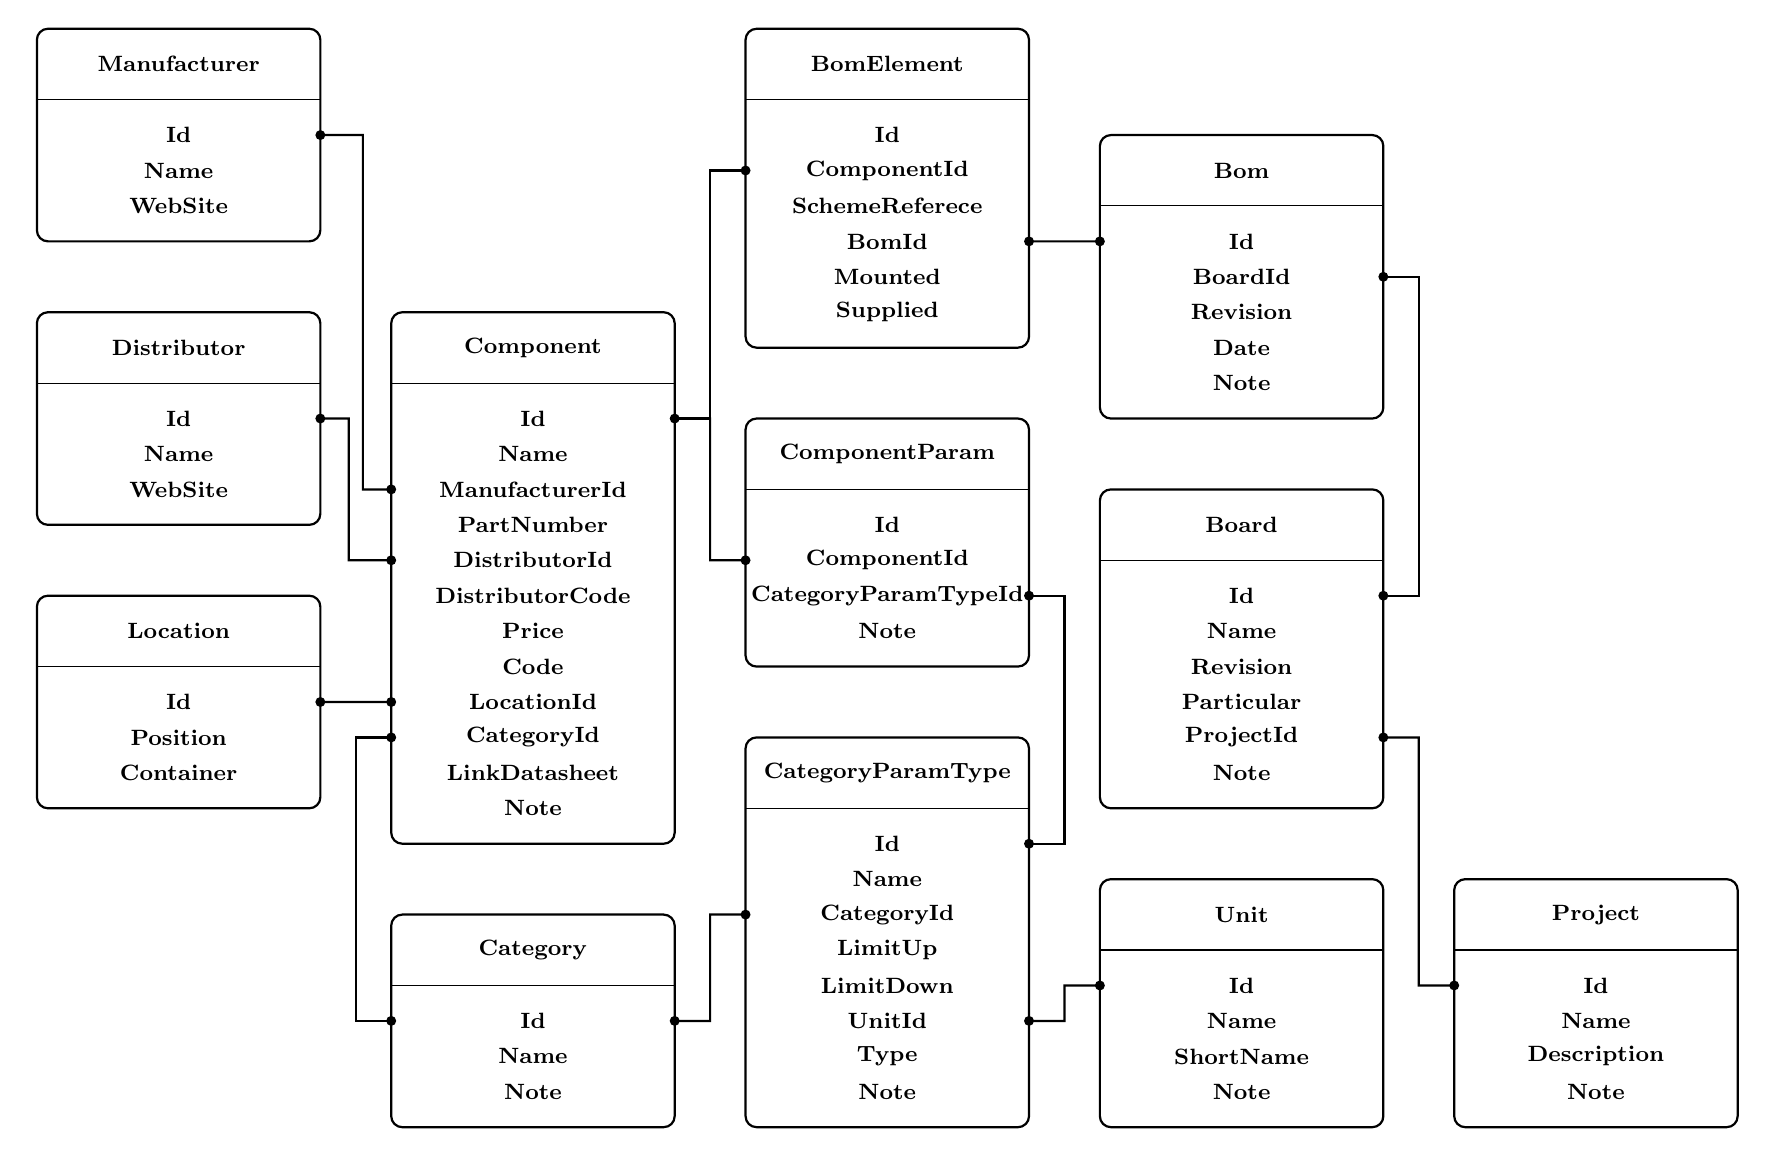
\begin{tikzpicture}[thick,scale=0.9]

% Component
\node (component) at (0,4){};
\draw[rounded corners] (component) rectangle ($(component)+(\tableblockwdth , \componentheight)$);
\node at ($(component)+(\tableblockcenter , \componentheight - 0.5)$) {\mysize{Component}}; 
\draw[thin]($(component)+(0 , \componentheight - 1)$)--($(component)+(\tableblockwdth , \componentheight - 1)$);
\node (component_id) at ($(component)+(\tableblockcenter , \componentheight - 1.5)$) {\mysize{Id}};
\node at ($(component)+(\tableblockcenter , \componentheight - 2)$) {\mysize{Name}};
\node (component_manufacturerid) at ($(component)+(\tableblockcenter , \componentheight - 2.5)$) {\mysize{ManufacturerId}};
\node at ($(component)+(\tableblockcenter , \componentheight - 3)$) {\mysize{PartNumber}};
\node (component_distributorid) at ($(component)+(\tableblockcenter , \componentheight - 3.5)$) {\mysize{DistributorId}};
\node at ($(component)+(\tableblockcenter , \componentheight - 4)$) {\mysize{DistributorCode}};
\node at ($(component)+(\tableblockcenter , \componentheight - 4.5)$) {\mysize{Price}};
\node at ($(component)+(\tableblockcenter , \componentheight - 5)$) {\mysize{Code}};
\node (component_locationid) at ($(component)+(\tableblockcenter , \componentheight - 5.5)$) {\mysize{LocationId}};
\node (component_categoryid) at ($(component)+(\tableblockcenter , \componentheight - 6)$) {\mysize{CategoryId}};
\node at ($(component)+(\tableblockcenter , \componentheight - 6.5)$) {\mysize{LinkDatasheet}};
\node at ($(component)+(\tableblockcenter , \componentheight - 7)$) {\mysize{Note}};

% Category
\node (category) at (0,0){};
\draw[rounded corners] (category) rectangle ($(category)+(\tableblockwdth , \categoryheight)$);
\node at ($(category)+(\tableblockcenter , \categoryheight - 0.5)$) {\mysize{Category}}; 
\draw[thin]($(category)+(0 , \categoryheight - 1)$)--($(category)+(\tableblockwdth , \categoryheight - 1)$);
\node (category_id) at ($(category)+(\tableblockcenter , \categoryheight - 1.5)$) {\mysize{Id}};
\node at ($(category)+(\tableblockcenter , \categoryheight - 2)$) {\mysize{Name}};
\node at ($(category)+(\tableblockcenter , \categoryheight - 2.5)$) {\mysize{Note}};

% ComponentParam
\node (componentparam) at (5,6.5){};
\draw[rounded corners] (componentparam) rectangle ($(componentparam)+(\tableblockwdth ,\componentparamheight)$);
\node at ($(componentparam)+(\tableblockcenter,\componentparamheight - 0.5)$) {\mysize{ComponentParam}}; 
\draw[thin]($(componentparam)+(0,\componentparamheight - 1)$)--($(componentparam)+(\tableblockwdth , \componentparamheight - 1)$);
\node at ($(componentparam)+(\tableblockcenter,\componentparamheight - 1.5)$) {\mysize{Id}};
\node (componentparam_componentid) at ($(componentparam)+(\tableblockcenter,\componentparamheight - 2)$) {\mysize{ComponentId}};
\node (componentparam_categoryparamtypeid) at ($(componentparam)+(\tableblockcenter,\componentparamheight - 2.5)$) {\mysize{CategoryParamTypeId}};
\node at ($(componentparam)+(\tableblockcenter,\componentparamheight - 3)$) {\mysize{Note}};

% CategoryParamType
\node (categoryparamtype) at (5,0){};
\draw[rounded corners] (categoryparamtype) rectangle ($(categoryparamtype)+(\tableblockwdth , \categoryparamtypeheight)$);
\node at ($(categoryparamtype)+(\tableblockcenter , \categoryparamtypeheight - 0.5)$) {\mysize{CategoryParamType}}; 
\draw[thin]($(categoryparamtype)+(0,\categoryparamtypeheight - 1)$)--($(categoryparamtype)+(\tableblockwdth , \categoryparamtypeheight - 1)$);
\node (categoryparamtype_id) at ($(categoryparamtype)+(\tableblockcenter , \categoryparamtypeheight - 1.5)$) {\mysize{Id}};
\node at ($(categoryparamtype)+(\tableblockcenter , \categoryparamtypeheight - 2)$) {\mysize{Name}};
\node (categoryparamtype_categoryid) at ($(categoryparamtype)+(\tableblockcenter , \categoryparamtypeheight - 2.5)$) {\mysize{CategoryId}};
\node at ($(categoryparamtype)+(\tableblockcenter , \categoryparamtypeheight - 3)$) {\mysize{LimitUp}};
\node at ($(categoryparamtype)+(\tableblockcenter , \categoryparamtypeheight - 3.5)$) {\mysize{LimitDown}};
\node (categoryparamtype_unitid) at ($(categoryparamtype)+(\tableblockcenter , \categoryparamtypeheight - 4)$) {\mysize{UnitId}};
\node at ($(categoryparamtype)+(\tableblockcenter , \categoryparamtypeheight - 4.5)$) {\mysize{Type}};
\node at ($(categoryparamtype)+(\tableblockcenter , \categoryparamtypeheight - 5)$) {\mysize{Note}};
	
% Unit
\node (unit) at (10,0){};
\draw[rounded corners] (unit) rectangle ($(unit)+(\tableblockwdth , \unitheight)$);
\node at ($(unit)+(\tableblockcenter , \unitheight - 0.5)$) {\mysize{Unit}}; 
\draw[thin]($(unit)+(0 , \unitheight - 1)$)--($(unit)+(\tableblockwdth , \unitheight - 1)$);
\node (unit_id) at ($(unit)+(\tableblockcenter , \unitheight - 1.5)$) {\mysize{Id}};
\node at ($(unit)+(\tableblockcenter , \unitheight - 2)$) {\mysize{Name}};
\node at ($(unit)+(\tableblockcenter , \unitheight - 2.5)$) {\mysize{ShortName}};
\node at ($(unit)+(\tableblockcenter , \unitheight - 3)$) {\mysize{Note}};

% BomElement
\node (bomelement) at (5,11){};
\draw[rounded corners] (bomelement) rectangle ($(bomelement)+(\tableblockwdth , \bomelementheight)$);
\node at ($(bomelement)+(\tableblockcenter , \bomelementheight - 0.5)$) {\mysize{BomElement}}; 
\draw[thin]($(bomelement)+(0 , \bomelementheight - 1)$)--($(bomelement)+(\tableblockwdth , \bomelementheight - 1)$);
\node at ($(bomelement)+(\tableblockcenter , \bomelementheight - 1.5)$) {\mysize{Id}};
\node (bomelement_componentid) at ($(bomelement)+(\tableblockcenter , \bomelementheight - 2)$) {\mysize{ComponentId}};
\node at ($(bomelement)+(\tableblockcenter , \bomelementheight - 2.5)$) {\mysize{SchemeReferece}};
\node (bomelement_bomid) at ($(bomelement)+(\tableblockcenter , \bomelementheight - 3)$) {\mysize{BomId}};
\node at ($(bomelement)+(\tableblockcenter , \bomelementheight - 3.5)$) {\mysize{Mounted}};
\node at ($(bomelement)+(\tableblockcenter , \bomelementheight - 4)$) {\mysize{Supplied}};

% Bom
\node (bom) at (10,10){};
\draw[rounded corners] (bom) rectangle ($(bom)+(\tableblockwdth , \bomheight)$);
\node at ($(bom)+(\tableblockcenter , \bomheight - 0.5)$) {\mysize{Bom}}; 
\draw[thin]($(bom)+(0 , \bomheight - 1)$)--($(bom)+(\tableblockwdth , \bomheight - 1)$);
\node (bom_id) at ($(bom)+(\tableblockcenter , \bomheight - 1.5)$) {\mysize{Id}};
\node (bom_boardid) at ($(bom)+(\tableblockcenter , \bomheight - 2)$) {\mysize{BoardId}};
\node at ($(bom)+(\tableblockcenter , \bomheight - 2.5)$) {\mysize{Revision}};
\node at ($(bom)+(\tableblockcenter , \bomheight - 3)$) {\mysize{Date}};
\node at ($(bom)+(\tableblockcenter , \bomheight - 3.5)$) {\mysize{Note}};

% Board
\node (board) at (10,4.5){};
\draw[rounded corners] (board) rectangle ($(board)+(\tableblockwdth , \boardheight)$);
\node at ($(board)+(\tableblockcenter , \boardheight - 0.5)$) {\mysize{Board}}; 
\draw[thin]($(board)+(0 , \boardheight - 1)$)--($(board)+(\tableblockwdth , \boardheight - 1)$);
\node (board_id) at ($(board)+(\tableblockcenter , \boardheight - 1.5)$) {\mysize{Id}};
\node at ($(board)+(\tableblockcenter , \boardheight - 2)$) {\mysize{Name}};
\node at ($(board)+(\tableblockcenter , \boardheight - 2.5)$) {\mysize{Revision}};
\node at ($(board)+(\tableblockcenter , \boardheight - 3)$) {\mysize{Particular}};
\node (board_projectid) at ($(board)+(\tableblockcenter , \boardheight - 3.5)$) {\mysize{ProjectId}};
\node at ($(board)+(\tableblockcenter , \boardheight - 4)$) {\mysize{Note}};

% Project
\node (project) at (15,0){};
\draw[rounded corners] (project) rectangle ($(project)+(\tableblockwdth , \projectheight)$);
\node at ($(project)+(\tableblockcenter , \projectheight - 0.5)$) {\mysize{Project}}; 
\draw[thin]($(project)+(0 , \projectheight - 1)$)--($(project)+(\tableblockwdth , \projectheight - 1)$);
\node (project_id) at ($(project)+(\tableblockcenter , \projectheight - 1.5)$) {\mysize{Id}};
\node at ($(project)+(\tableblockcenter , \projectheight - 2)$) {\mysize{Name}};
\node at ($(project)+(\tableblockcenter , \projectheight - 2.5)$) {\mysize{Description}};
\node at ($(project)+(\tableblockcenter , \projectheight - 3)$) {\mysize{Note}};

% Location
\node (location) at (-5,4.5){};
\draw[rounded corners] (location) rectangle ($(location)+(\tableblockwdth , \locationheight)$);
\node at ($(location)+(\tableblockcenter , \locationheight - 0.5)$) {\mysize{Location}}; 
\draw[thin]($(location)+(0 , \locationheight - 1)$)--($(location)+(\tableblockwdth , \locationheight - 1)$);
\node (location_id) at ($(location)+(\tableblockcenter , \locationheight - 1.5)$) {\mysize{Id}};
\node at ($(location)+(\tableblockcenter , \locationheight - 2)$) {\mysize{Position}};
\node at ($(location)+(\tableblockcenter , \locationheight - 2.5)$) {\mysize{Container}};

% Distributor
\node (distributor) at (-5,8.5){};
\draw[rounded corners] (distributor) rectangle ($(distributor)+(\tableblockwdth , \distributorheight)$);
\node at ($(distributor)+(\tableblockcenter , \distributorheight - 0.5)$) {\mysize{Distributor}}; 
\draw[thin]($(distributor)+(0 , \distributorheight - 1)$)--($(distributor)+(\tableblockwdth , \distributorheight - 1)$);
\node (distributor_id) at ($(distributor)+(\tableblockcenter , \distributorheight - 1.5)$) {\mysize{Id}};
\node at ($(distributor)+(\tableblockcenter , \distributorheight - 2)$) {\mysize{Name}};
\node at ($(distributor)+(\tableblockcenter , \distributorheight - 2.5)$) {\mysize{WebSite}};

% Manufacturer
\node (manufacturer) at (-5,12.5){};
\draw[rounded corners] (manufacturer) rectangle ($(manufacturer)+(\tableblockwdth , \manufacturerheight)$);
\node at ($(manufacturer)+(\tableblockcenter , \manufacturerheight - 0.5)$) {\mysize{Manufacturer}}; 
\draw[thin]($(manufacturer)+(0 , \manufacturerheight - 1)$)--($(manufacturer)+(\tableblockwdth , \manufacturerheight - 1)$);
\node (manufacturer_id) at ($(manufacturer)+(\tableblockcenter , \manufacturerheight - 1.5)$) {\mysize{Id}};
\node at ($(manufacturer)+(\tableblockcenter , \manufacturerheight - 2)$) {\mysize{Name}};
\node at ($(manufacturer)+(\tableblockcenter , \manufacturerheight - 2.5)$) {\mysize{WebSite}};

%%%%%%%%%%%%%%%%%%%%%%%%%%%%%%%%%%%%%%%
% Points
\fill ($(category_id) - (\tableblockcenter ,0)$) circle (2pt);
\fill ($(category_id) + (\tableblockcenter ,0)$) circle (2pt);

\fill ($(component_id) + (\tableblockcenter ,0)$) circle (2pt);
\fill ($(component_categoryid) - (\tableblockcenter ,0)$) circle (2pt);
\fill ($(component_locationid) - (\tableblockcenter ,0)$) circle (2pt);
\fill ($(component_distributorid) - (\tableblockcenter ,0)$) circle (2pt);
\fill ($(component_manufacturerid) - (\tableblockcenter ,0)$) circle (2pt);

\fill ($(componentparam_componentid) - (\tableblockcenter ,0)$) circle (2pt);
\fill ($(componentparam_categoryparamtypeid) + (\tableblockcenter ,0)$) circle (2pt);

\fill ($(categoryparamtype_id) + (\tableblockcenter ,0)$) circle (2pt);
\fill ($(categoryparamtype_categoryid) - (\tableblockcenter ,0)$) circle (2pt);
\fill ($(categoryparamtype_unitid) + (\tableblockcenter ,0)$) circle (2pt);

\fill ($(unit_id) - (\tableblockcenter ,0)$) circle (2pt);

\fill ($(bomelement_componentid) - (\tableblockcenter ,0)$) circle (2pt);
\fill ($(bomelement_bomid) + (\tableblockcenter ,0)$) circle (2pt);

\fill ($(bom_id) - (\tableblockcenter ,0)$) circle (2pt);
\fill ($(bom_boardid) + (\tableblockcenter ,0)$) circle (2pt);

\fill ($(board_id) + (\tableblockcenter ,0)$) circle (2pt);
\fill ($(board_projectid) + (\tableblockcenter ,0)$) circle (2pt);

\fill ($(project_id) - (\tableblockcenter ,0)$) circle (2pt);

\fill ($(location_id) + (\tableblockcenter ,0)$) circle (2pt);

\fill ($(distributor_id) + (\tableblockcenter ,0)$) circle (2pt);

\fill ($(manufacturer_id) + (\tableblockcenter ,0)$) circle (2pt);

%%%%%%%%%%%%%%%%%%%%%%%%%%%%%%%%%%%%%%%
% Line
\draw ($(component_categoryid) - (\tableblockcenter , 0)$) -- ($(component_categoryid) - (\tableblockcenter + 0.5,0)$) -- ($(category_id) - (\tableblockcenter + 0.5,0)$) -- ($(category_id) - (\tableblockcenter ,0)$) ; 
\draw ($(location_id) + (\tableblockcenter , 0)$) -- ($(location_id) + (\tableblockcenter + 0.5,0)$) -- ($(component_locationid) - (\tableblockcenter + 0.5,0)$) -- ($(component_locationid) - (\tableblockcenter ,0)$) ; 
\draw ($(distributor_id) + (\tableblockcenter , 0)$) -- ($(distributor_id) + (\tableblockcenter + 0.4,0)$) -- ($(component_distributorid) - (\tableblockcenter + 0.6,0)$) -- ($(component_distributorid) - (\tableblockcenter ,0)$) ; 
\draw ($(manufacturer_id) + (\tableblockcenter , 0)$) -- ($(manufacturer_id) + (\tableblockcenter + 0.6,0)$) -- ($(component_manufacturerid) - (\tableblockcenter + 0.4,0)$) -- ($(component_manufacturerid) - (\tableblockcenter ,0)$) ; 

\draw ($(categoryparamtype_categoryid) - (\tableblockcenter , 0)$) -- ($(categoryparamtype_categoryid) - (\tableblockcenter + 0.5,0)$) -- ($(category_id) + (\tableblockcenter + 0.5,0)$) -- ($(category_id) + (\tableblockcenter ,0)$) ; 

\draw ($(componentparam_componentid) - (\tableblockcenter , 0)$) -- ($(componentparam_componentid) - (\tableblockcenter + 0.5,0)$) -- ($(component_id) + (\tableblockcenter + 0.5,0)$) -- ($(component_id) + (\tableblockcenter ,0)$) ; 
\draw ($(bomelement_componentid) - (\tableblockcenter , 0)$) -- ($(bomelement_componentid) - (\tableblockcenter + 0.5,0)$) |- ($(component_id) + (\tableblockcenter + 0.5,0)$) -- ($(component_id) + (\tableblockcenter ,0)$) ; 

\draw ($(categoryparamtype_id) + (\tableblockcenter , 0)$) -- ($(categoryparamtype_id) + (\tableblockcenter + 0.5,0)$) -- ($(componentparam_categoryparamtypeid) + (\tableblockcenter + 0.5,0)$) -- ($(componentparam_categoryparamtypeid) + (\tableblockcenter ,0)$) ; 

\draw ($(categoryparamtype_unitid) + (\tableblockcenter , 0)$) -- ($(categoryparamtype_unitid) + (\tableblockcenter + 0.5,0)$) -- ($(unit_id) - (\tableblockcenter + 0.5,0)$) -- ($(unit_id) - (\tableblockcenter ,0)$) ; 

\draw ($(bomelement_bomid) + (\tableblockcenter , 0)$) -- ($(bomelement_bomid) + (\tableblockcenter + 0.5,0)$) -- ($(bom_id) - (\tableblockcenter + 0.5,0)$) -- ($(bom_id) - (\tableblockcenter ,0)$) ; 

\draw ($(bom_boardid) + (\tableblockcenter , 0)$) -- ($(bom_boardid) + (\tableblockcenter + 0.5,0)$) -- ($(board_id) + (\tableblockcenter + 0.5,0)$) -- ($(board_id) + (\tableblockcenter ,0)$) ; 

\draw ($(board_projectid) + (\tableblockcenter , 0)$) -- ($(board_projectid) + (\tableblockcenter + 0.5,0)$) -- ($(project_id) - (\tableblockcenter + 0.5,0)$) -- ($(project_id) - (\tableblockcenter ,0)$) ; 

\end{tikzpicture}
\end{document}